%\section{New technique or technique adaptation}
\section{Alinhamento Semi - automático}
\label{sec:technique}

\subsection{Iterative Closest Point}

Um dos grandes problemas no desenvolvimento de reconstrução de malhas, com certeza se caracteriza pelo alinhamento de duas malhas parcialmente sobrepostas; com dados pontos iniciais correspondentes para uma relativa transformação.

Para nos auxiliar no problema de alinhamento em relação às duas malhas, utilizamos o algoritmo \textit{Iterative Closest Point} (ICP) \cite{Zhang:1994}; que nos fornece à minimização da distância de cada ponto de uma malha D, a cada ponto correspondente de cada malha M.

\subsection{Iterative Closest Point}

Um dos grandes problemas no desenvolvimento de reconstrução de malhas, com certeza se caracteriza pelo alinhamento de duas malhas parcialmente sobrepostas; com dados pontos iniciais correspondentes para uma relativa transformação.

Para nos auxiliar no problema de alinhamento em relação às duas malhas, utilizamos o algoritmo \textit{Iterative Closest Point} (ICP) \cite{Zhang:1994}; que nos fornece à minimização da distância de cada ponto de uma malha D, a cada ponto correspondente de cada malha M.

Para o nosso problema, utilizamos um conjunto de passos para resolve-los. Inicialmente escolhemos nosso conjunto de vertíces de uma malha M, que apresenta seu respectivo correspondente à malha D; Segue \ref{ICP} como imagem. Após esse passo, utilizamos o cálculo dos centroides em relação à cada malha. Em seguida, desenvolvemos o cálculo do alinhamento, aonde envolvemos os principais operadores de transformação(rotação e translação, respectivamente) em relação à cada conjunto de correspondências entre M e D, na qual nos retorna uma matriz de transformação; e por fim aplicamos o alinhamento, utilizando a matriz de transformação em relação à malha que sofre a sobreposição.

\begin{figure}[h]
\center
    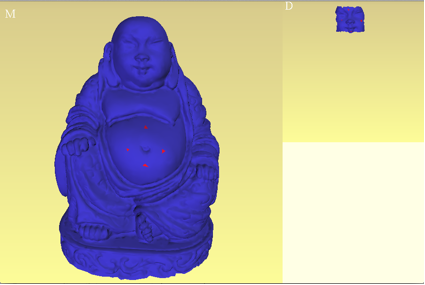
\includegraphics[width=8cm]{ImagemICP2}
        \label{ICP}
\end{figure}
\vspace{4mm}

\subsection{Parametrização conforme}

Para nos facilitar na classificação do método de parametrização, utilizamos uma técnica de bordo livre, com foco em deformação para análise complexa. Com isso, aplicamos a parametrização espectral de \cite{Mullen} nas duas malhas, mantendo como restrição que os vértices correspondentes sejam mapeados para as mesmas coordenadas paramétricas.

%$\mathbb{R}^{3} \longrightarrow \mathbb{R}^2$,
Para isso, inicialmente aplicamos uma projeção em ambas malhas no intuito de encontrar o menor eixo do \textit{bounding box}, e "prender" os vértices extremos.
 
Posteriormente, utilizamos uma técnica conhecida como LSCM (\textit{Least Squares Conformal Maps}) \cite{Levy:2002}; que tem o objetivo em minimizar a energia conforme, devido as superfícies em geral não admitirem parametrização conforme.

A minimização M se caracteriza pela seguinte equação:
\[ M = \sum_{T}= \left|\left| \left[ \begin{array}{c}  \dfrac{\partial v}{\partial x} \\ \\  \dfrac{\partial v}{\partial y}  \end{array} \right] - \left[ \begin{array}{c}  -\dfrac{\partial u}{\partial y}  \\ \\ \dfrac{\partial u}{\partial x}  \end{array} \right] \right| \right|^{2} \]
\vspace*{0.3mm}

Mantendo dois vértices para determinar a rotação, translação e escalonamento.

E por fim. aplicamos um algoritmo, conhecido como \textit{Thin Plane Spline} \cite{Duchon} que nos favorece a interpolação necessária para formação da parametrização 2D.
%
%Our technique aims at obtaining that result. It particularly suits to the problem since it is formulated as\ldots{}


%%------------------------------------------------------------------------- 
%\subsection{Formulation}
%
%
%%------------------------------------------------------------------------- 
%\subsection{Solution}
%
%
%%------------------------------------------------------------------------- 
%\subsection{Initialization and tuning}